% -*- coding: utf-8 -*-
% !TEX program = xelatex
\documentclass{jnuthesis}
\usepackage{amsmath}
\usepackage{algorithmic}
\usepackage{array}
\usepackage{fixltx2e}
\usepackage{stfloats}
\usepackage{url}
\usepackage{multicol}
\usepackage{graphicx}
\usepackage{ctex}
\usepackage{subfigure}
\usepackage{float}
\usepackage{indentfirst}
\usepackage{booktabs}
\usepackage{lscape}
\usepackage{caption}
\usepackage{subfigure}
%\usepackage[backend=biber,style=gb7714-2015]{biblatex}
%\usepackage[super]{gbt7714}
\usepackage{gbt7714}
\usepackage{titlesec}\titleclass{\chapter}{straight}
\titleformat{\chapter}[hang]  {\huge\bfseries}{\arabic{chapter}}{1em}{}

\usepackage{listings}
\usepackage{xcolor} 


\definecolor{mygreen}{rgb}{0,0.6,0}
\definecolor{mygray}{rgb}{0.5,0.5,0.5}
\definecolor{mymauve}{rgb}{0.58,0,0.82}
\lstset{ %
	backgroundcolor=\color{white},   % choose the background color
	basicstyle=\footnotesize\ttfamily,        % size of fonts used for the code
	columns=fullflexible,
	breaklines=true,                 % automatic line breaking only at whitespace
	captionpos=b,                    % sets the caption-position to bottom
	tabsize=4,
	commentstyle=\color{mygreen},    % comment style
	escapeinside={\%*}{*)},          % if you want to add LaTeX within your code
	keywordstyle=\color{blue},       % keyword style
	stringstyle=\color{mymauve}\ttfamily,     % string literal style
	frame=shadowbox,
	rulesepcolor=\color{red!20!green!20!blue!20},
	% identifierstyle=\color{red},
	numbers=left, 
	numberstyle=\tiny,
	% escapeinside=' ',
	xleftmargin=2em,
	xrightmargin=2em, 
	aboveskip=1em
}

\begin{document}

\renewcommand{\title}{A thesis class for Jinan University} % 英文标题
\renewcommand{\biaoti}{基于GRU的股市预测}  % 中文标题
\renewcommand{\xueyuan}{国际能源学院}
\renewcommand{\zhuanye}{电气工程及其自动化}
\renewcommand{\xingming}{余思贤、周允康}
\renewcommand{\xuehao}{2018054439}
\renewcommand{\daoshi}{庄师强}
\renewcommand{\zuzhang}{苏日清}
\renewcommand{\zuyuanone}{余思贤}
\renewcommand{\zuyuantwo}{梁宗威}
\renewcommand{\zuyuanthree}{谭铭濠}
\renewcommand{\zuyuanxhone}{2018054439}
\renewcommand{\zuyuanxhtwo}{2018054439}
\renewcommand{\zuyuanxhthree}{2018054439}
\renewcommand{\zuzhangxh}{2018054439}

\titlepage





\chapter{课程设计的任务与要求}
\section{课程设计的任务}

\begin{enumerate}
	\item 熟悉MATLAB中深度学习工具箱的使用方法,喂入数据的方法,配置训练的方法,保存模型的方法和调用模型的方法;
	\item 能画出学习模型的基本框架,理解其基本原理;
	\item 基于GRU对中国石化的开盘股价进行预测。
\end{enumerate}




\section{课程设计的要求}
\begin{enumerate}
	\item 学会MATLAB软件的安装;
	\item 熟练掌握MATLAB的使用,掌握深度学习工具箱的使用;
	\item 能使用深度学习工具箱根据需求搭建神经网络,喂入数据,训练,得出模型并能调用;
	\item 通过调参使得模型能更好的贴合实际,打到更好的效果。
\end{enumerate}

\chapter{研究基础}
\section{序列数据神经网络}

\subsection{RNN网络}
循环神经网络(Recurrent Neural Network,RNN)是一种用于处理序列数据的神经网络。相比一般的神经网络来说,他能够处理序列变化的数据。比如某个单词的意思会因为上文提到的内容不同而有不同的含义,RNN就能够很好地解决这类问题。

一般来说,普通RNN网络形式如下:
\begin{align}
	h^{\prime}=&\delta(w_h h+w_i x+b^{h})\\
	 y=&\delta( w_o h^{\prime}+b^{y})
\end{align}


其中$ h^{\prime} $为传入下一节点的参数,$ y $常使用对$ h^{\prime} $进行唯独映射,然后使用$ softmax $进行分类得到所需的参数。


\begin{figure}[H]
	\centering
	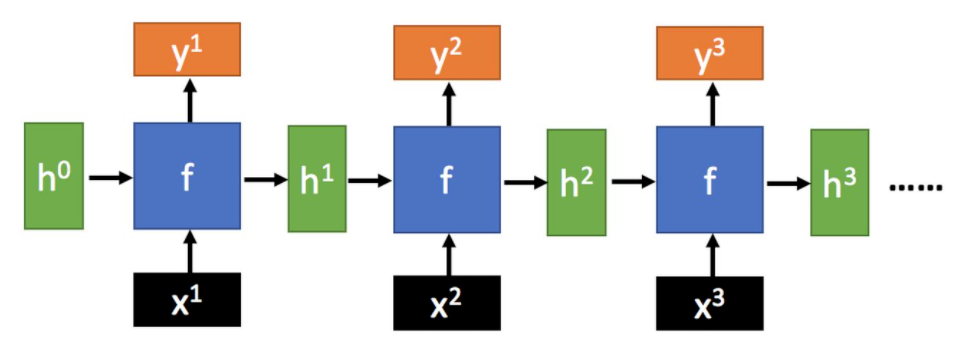
\includegraphics[width=\linewidth]{pic/screenshot001}
	\caption{多级RNN网络构成}
	\label{fig:screenshot001}
\end{figure}

\subsection{LSTM结构}

长短期记忆(Long short-term memory, LSTM)是一种特殊的RNN,主要是为了解决长序列训练过程中的梯度消失和梯度爆炸问题。简单来说,就是相比普通的RNN,LSTM能够在更长的序列中有更好的表现。

\begin{figure}[H]
	\centering
	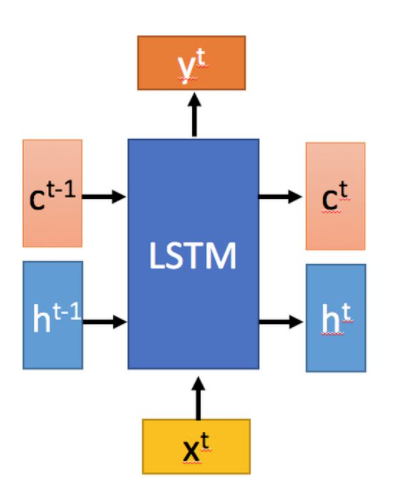
\includegraphics[width=0.3\linewidth]{pic/screenshot002}
	\caption{LTSM网络结构}
	\label{fig:screenshot002}
\end{figure}

LSTM网络的表达式如下:
\begin{align}
	 c^t=&z^f\odot c^{t-1}+z^{i}\odot z\\
	 h^{t}=&z^{o}\odot \tanh{c^{t}}\\
	 y^{t}=&\delta(W^{\prime}h^{t}+b^{y})
\end{align}

其中$ c^{t} $可以理解为长期记忆,主要是用来保存节点传递下来的数据的,每次传递会对某些维度进行“忘记”并且会加入当前节点所包含的内容;,$ h^{t} $则为短期记忆,仅保存了先前节点的信息。

\subsection{GRU网络}
GRU(Gate Recurrent Unit)是循环神经网络(Recurrent Neural Network, RNN)的一种。和LSTM(Long-Short Term Memory)一样,也是为了解决长期记忆和反向传播中的梯度等问题而提出来的。

GRU的输入输出结构与普通的RNN是一样的。
\begin{figure}[H]
	\centering
	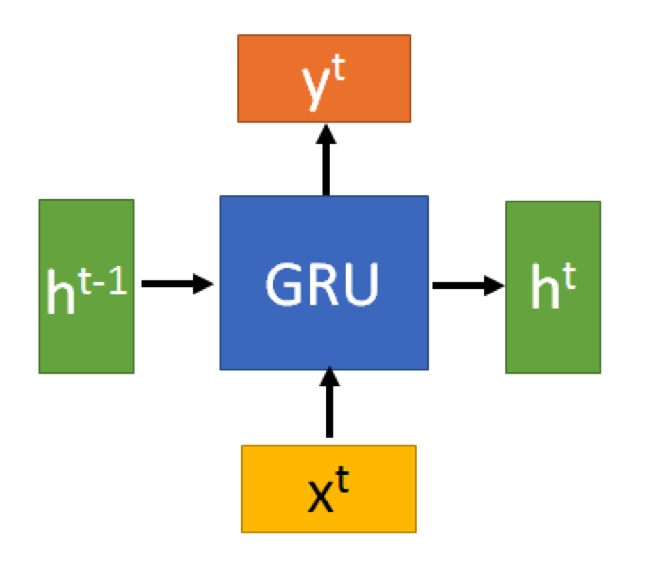
\includegraphics[width=0.3\linewidth]{pic/screenshot003}
	\caption{GRU的输入输出结构}
	\label{fig:screenshot003}
\end{figure}

其表达式为:
\begin{align}
	r^{t}=&\delta(x^{t}w^{xr}+h^{t-1}w^{hr}+b^{r})\\
	z^{t}=&\delta(x^{t}w^{xz}+h^{t-1}w^{hz}+b^{z})\\
	h^{\prime}=&\tanh{x^{t}w^{xr}+r^{t}\odot h^{t-1}w^{hh}+b^{h} }\\
	h^t=&(1-z)\odot h^{\prime}+z\odot h^{t-1}\\
	y^{t}=&\text{softmax}(h^{t}w^{hy}+b^{y})
\end{align}


GRU与LSTM相比,需要训练的参数较少,但也能达到与LSTM相近的效果。其训练的参数少,对硬件要求要求较低,因此本文采用GRU进行实现。
\section{训练数据的准备}
\subsection{数据采集}
这里使用Python爬取近16年中国石化(600028)的股市信息。

代码如下:

\begin{lstlisting} [language=Python]
import tushare as ts

df1 = ts.get_k_data('600028', ktype='D', start='2005-01-01', end='2021-10-16')

datapath1 = "./SH600028.csv"
df1.to_csv(datapath1)
\end{lstlisting}

得到了4032行数据,包括:时间、开盘价格、收市价、高位、低位、成交量以及股票代码。

\subsection{数据处理}

为使得模型更快收敛,并提高其准确性,对取得的数据进行归一化处理,公式如下:

\begin{equation}
x^*=\frac{X-X_{min}}{X_{max}-X_{min}}
\end{equation}


核心代码如下:
\begin{lstlisting} [language=Python]
from sklearn.preprocessing import MinMaxScaler

sc = MinMaxScaler(feature_range=(0, 1))  
training_set_scaled = sc.fit_transform(training_set)
test_set = sc.transform(test_set)
\end{lstlisting}

\subsection{数据标注}

为了实现股票预测,需要对训练用的数据进行标注。

GRU是根据过去预测未来,因此采用前两个月的数据进行对当日开盘价的预测。

取出后200日的数据作为测试数据,前3832日数据作为训练数据。

使用Python进行数据标注,并保存为txt文件,方便在MATLAB中进行读取调用。

标注核心代码如下:
\begin{lstlisting} [language=Python]
import pandas as pd

test_num=200
day=60

zhongshihua = pd.read_csv('./SH600028.csv')  
training_set = zhongshihua.iloc[0:len(zhongshihua) - test_num, 2:3].values
test_set = zhongshihua.iloc[len(zhongshihua) - test_num:, 2:3].values

for i in range(day, len(training_set_scaled)):  
	x_train.append(training_set_scaled[i - day:i, 0])
	y_train.append(training_set_scaled[i, 0])
\end{lstlisting}


\section{股市预测的Python实现}


先在Python中调用tensorflow框架进行本项目的实现,验证其可行性。

\begin{figure}[H]
	\centering
	
\includegraphics[width=1\linewidth]{pic/screenshot004}
	\caption{股市预测网络结构}
	\label{fig:screenshot004}
\end{figure}

核心代码如下(仅展示模型部分):
\begin{lstlisting} [language=Python]
import tensorflow as tf
from tensorflow.keras.layers import Dropout, Dense, GRU

model = tf.keras.Sequential([   
	GRU(512, return_sequences=True),
	Dropout(0.2),
	GRU(1024),
	Dropout(0.2),
	Dense(1)
	])
\end{lstlisting}


 第一层GRU:512个单元,每次返回$ h^t $参数;
 令其中20\%的单元休眠;
 第二层GRU:1024个单元,仅最后一次返回$ h^t $参数;
 令其中20\%的单元休眠;
 最后进行全链接输出。

在epochs=100,batch size=32的训练条件下,预测结果如图\ref{fig:screenshot005}:
\begin{figure}[H]
	\centering
	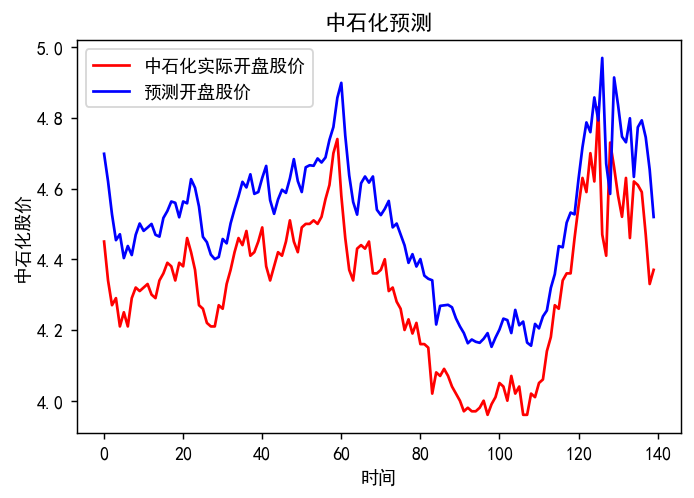
\includegraphics[width=0.7\linewidth]{pic/screenshot005}
	\caption{预测结果}
	\label{fig:screenshot005}
\end{figure}

可以看到:预测出的趋势与实际相比是较为准确的。

\chapter{股市预测的MATLAB实现}
\section{深度学习工具箱}

深度学习工具箱提供了一个用于通过算法、预训练模型和 App 来设计和实现深度神经网络的框架。在深度学习工具箱中可以使用卷积神经网络(ConvNet、CNN)和长短期记忆 (LSTM) 网络对图像、时序和文本数据执行分类和回归。可以使用自动微分、自定义训练循环和共享权重来构建网络架构,如生成对抗网络 (GAN) 和孪生网络。使用深度网络设计器,能够以图形方式设计、分析和训练网络。试验管理器可管理多个深度学习试验,跟踪训练参数,分析结果,并比较不同试验的代码。可以可视化层激活,并以图形方式监控训练进度。\cite{MathWorks}


下面代码架构均使用深度学习工具箱生成。
\section{在MATLAB中搭建GRU神经网络}



在深度学习工具箱中,可以快速搭建神经网络
\begin{figure}[H]
	\centering
	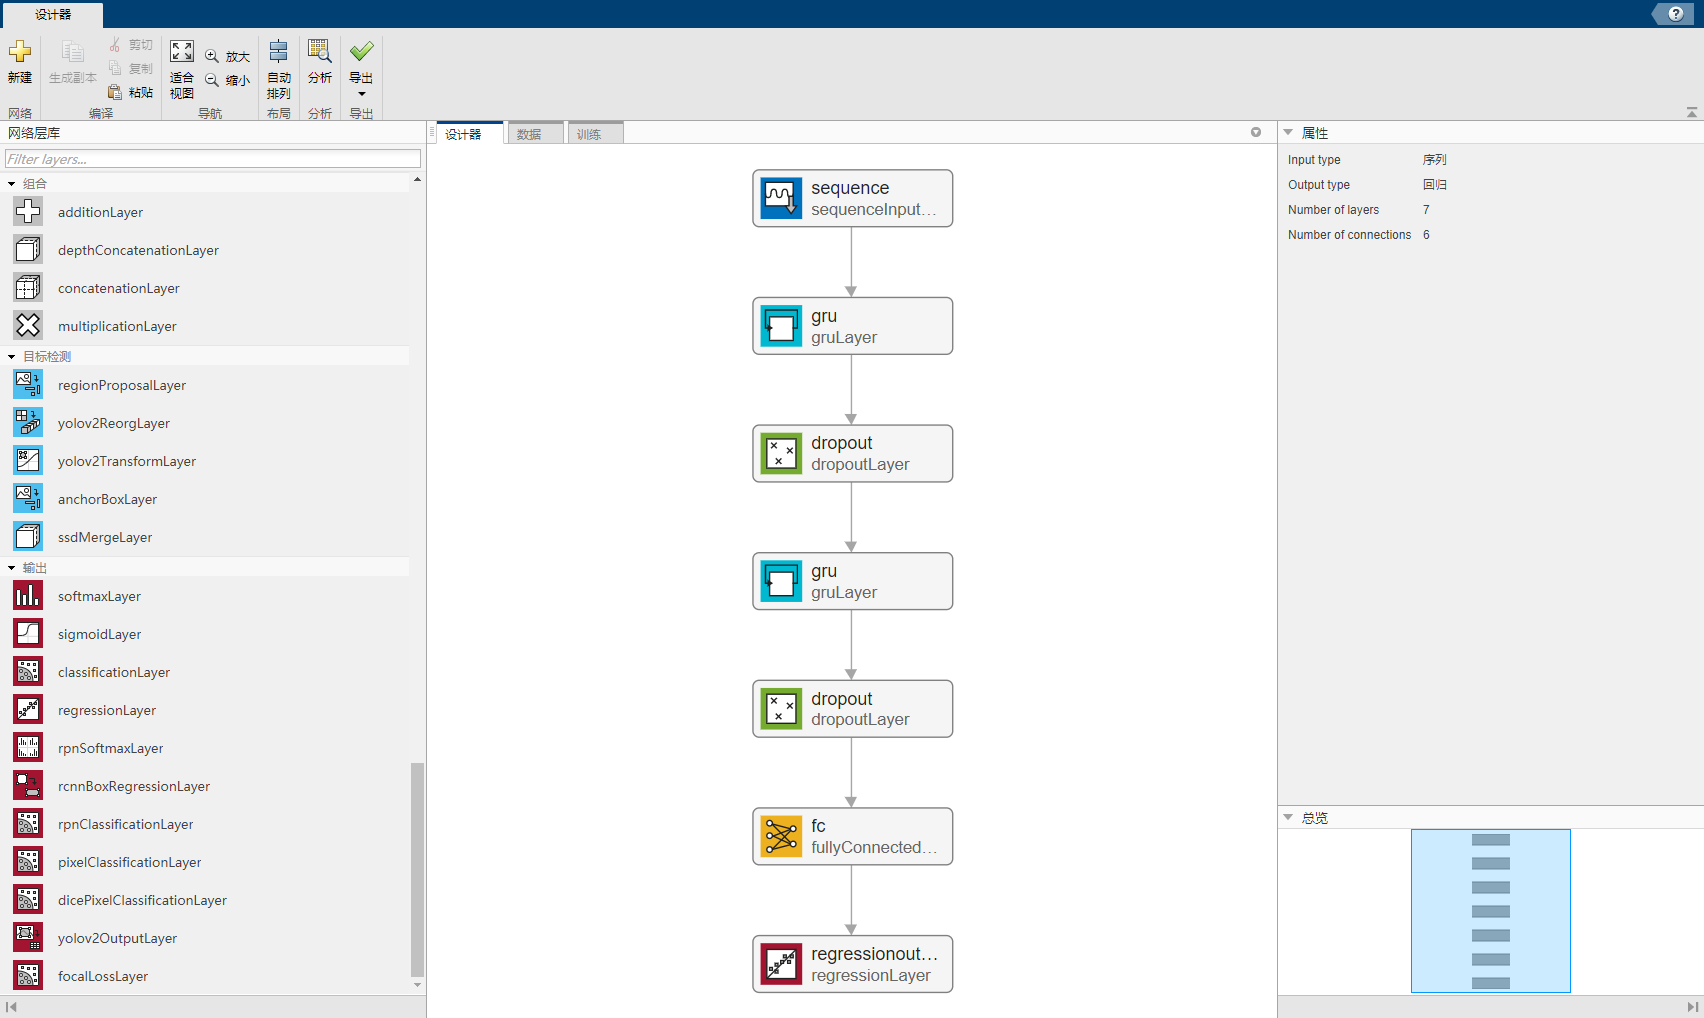
\includegraphics[width=0.8\linewidth]{pic/screenshot018}
	\caption{使用深度学习工具箱中快速搭建基础神经网络}
	\label{fig:screenshot017}
\end{figure}

通过深度学习工具箱,我们可以快速导出神经网络模型,得到结果如图\ref{fig:screenshot019}所示:
\begin{figure}[H]
	\centering
	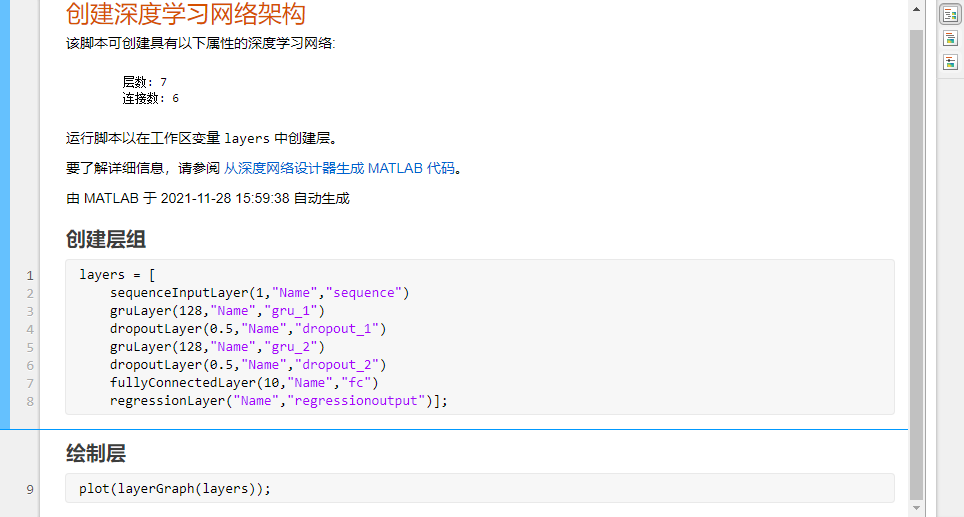
\includegraphics[width=0.7\linewidth]{pic/screenshot019}
	\caption{使用深度学习工具箱创建深度学习网络架构}
	\label{fig:screenshot019}
\end{figure}

在Matlab中,程序核心代码如下:

\begin{enumerate}
	\item 网络架构部分:

\begin{lstlisting} [language=Matlab]
function layers=get_gru_net(wd)
numFeatures=wd;
numResponses=1;
numHiddenUnits=512;

layers=[sequenceInputLayer(numFeatures)
	gruLayer(numHiddenUnits)
	dropoutLayer(0.2)
	gruLayer(2*numHiddenUnits)
	dropoutLayer(0.2)
	fullyConnectedLayer(numResponses)
	regressionLayer];
end
\end{lstlisting}

\item 模型超参数选项设置部分:
\begin{lstlisting} [language=Matlab]
layers=get_gru_net(wd);
options=trainingOptions('adam',...
	'MaxEpochs',100,...
	'GradientThreshold',1,...
	'InitialLearnRate',0.001, ...
	'LearnRateSchedule','piecewise',...
	'LearnRateDropPeriod',125,...
	'LearnRateDropFactor',0.2,...
	'Verbose',0,...
	'Plots','training-progress');
\end{lstlisting}
\end{enumerate}



\section{喂入数据并训练}

在Matlab中,使用函数$ trainNetwork $将数据喂入神经网络并训练。训练过程如图\ref{fig:screenshot015}所示:

\begin{figure}[H]
	\centering
	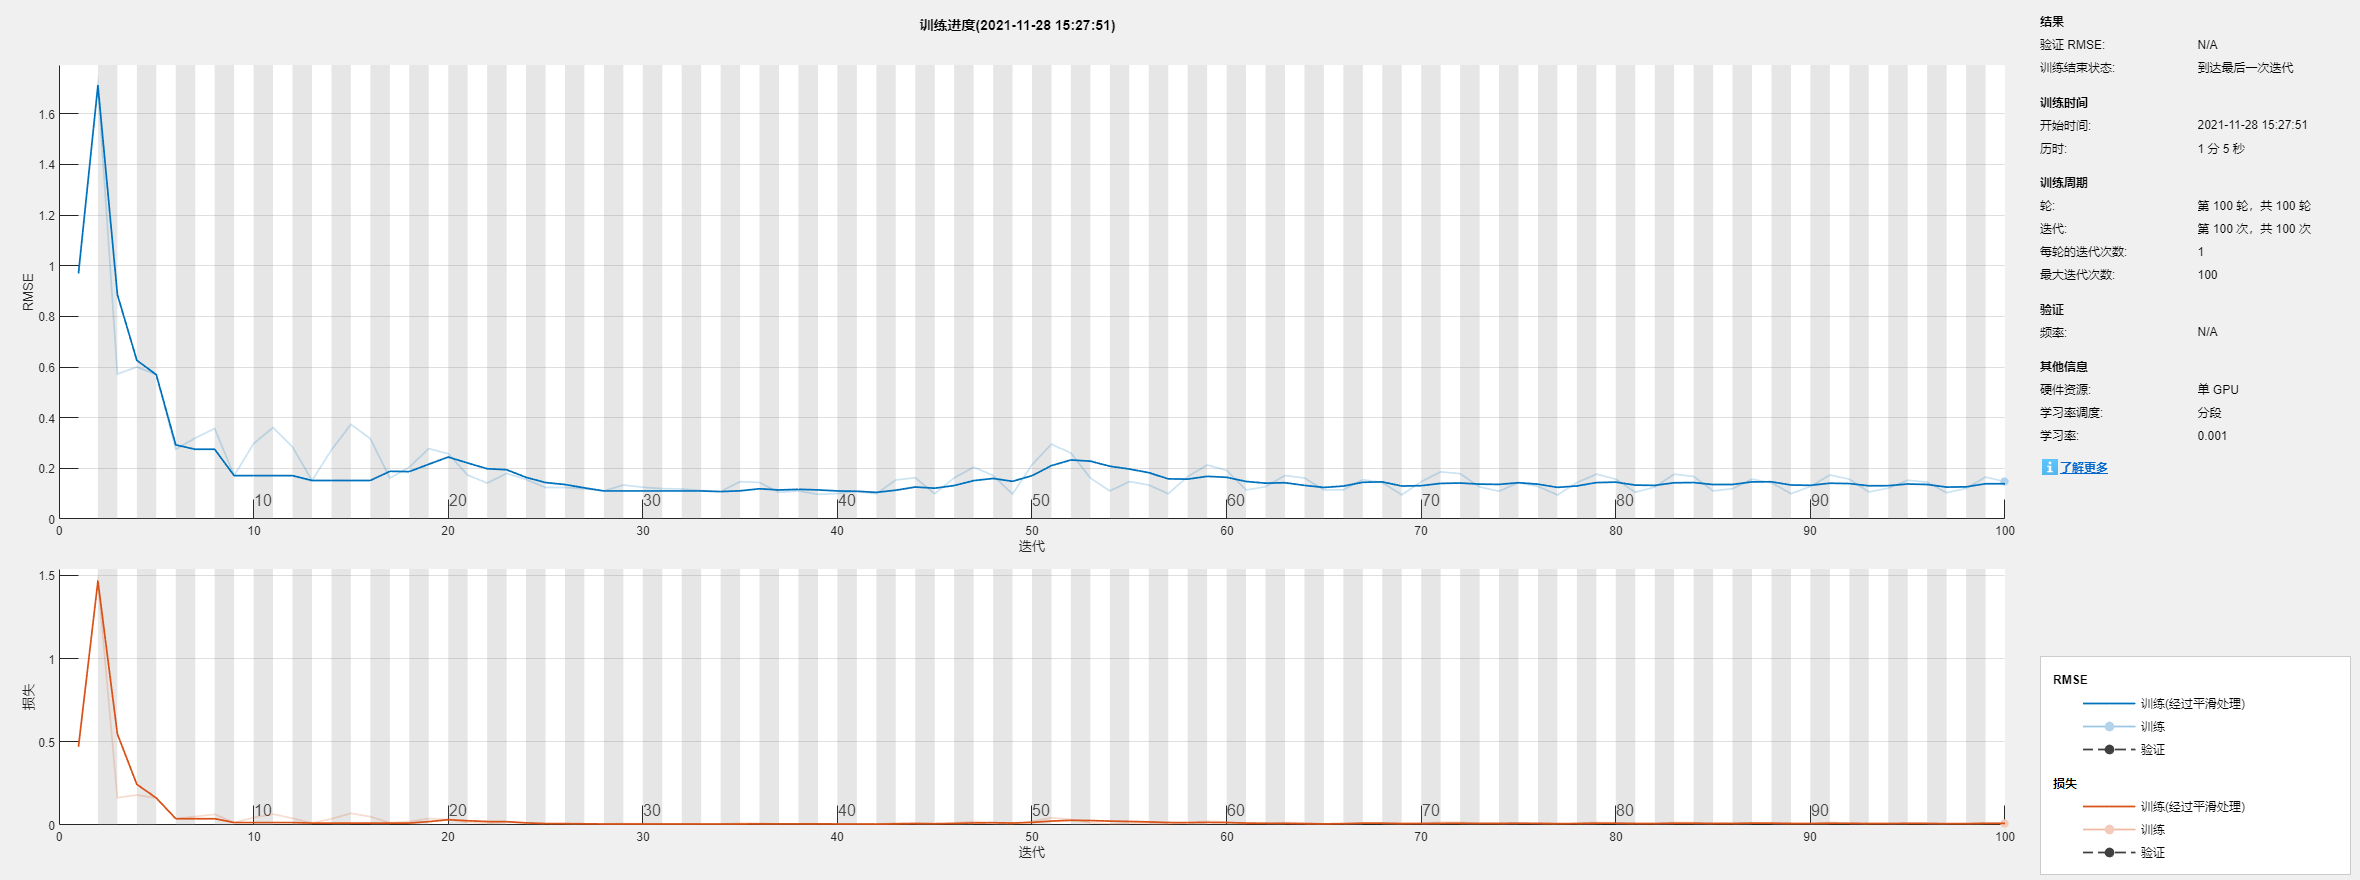
\includegraphics[width=1\linewidth]{pic/screenshot015}
	\caption{训练进度展示}
	\label{fig:screenshot015}
\end{figure}

使用函数$ predict $调用训练好的模型进行预测。此神经网络预测结果如图\ref{fig:screenshot016}所示:

\begin{figure}[H]
	\centering
	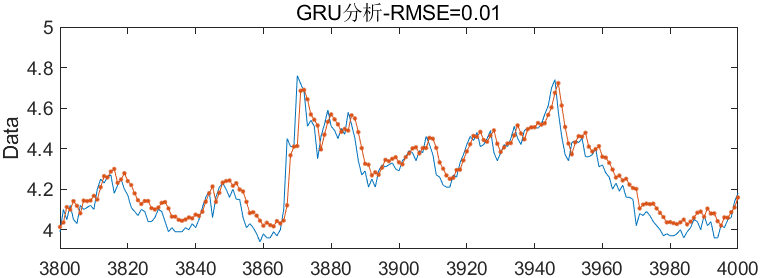
\includegraphics[width=1\linewidth]{pic/screenshot016}
	\caption{GRU预测结果:图中\textcolor[RGB]{217, 83, 25}{橘红色}曲线为预测数值, \textcolor[RGB]{97,167,212}{蓝色}为实际数值}
	\label{fig:screenshot016}
\end{figure}


\section{模型优化}


\subsection{效果评判}
后续测试模型中,我们采用茅台2005年1月1日到2021年3月20日的开盘股价作为训练集,为了节省时间,规定每一种模型均跑100Epoch。

我们使用如下指标进行模型效果评判:

\begin{enumerate}
	\item 计算茅台在2021年3月30日到2021年10月16日,共计200日的开盘股价预测数据,并与此200日的实际开盘股价计算确定系数。
	
	确定系数计算公式如下:
	\begin{equation}\label{r}
		r(X,Y)=\dfrac{\texttt{Cov}(X,Y)}{\sqrt{\texttt{Var}[X]\texttt{Var}[Y]}}
	\end{equation}
	式中,$ \texttt{Cov}(X,Y) $为X与Y的协方差,$ \texttt{Var}[X] $为X的方差,$ \texttt{Var}[Y] $为Y的方差。
	\item 计算模型计算速度,测试数据为:茅台在2021年3月30日到2021年10月16日的股价预测数据。计算速度测试中,时间计算单位为ms,一共跑100次,取平均值。
	\item 测试设备为联想拯救者R9000P(5800H+64G内存+RTX3070-8G)
	
	\item 综合评判公式:
	
	\begin{equation}\label{pingpan}
		s=\dfrac{100r}{T}
	\end{equation}
\end{enumerate}


\subsection{更改模型}
在3.3中,我们得到了粗略的结果,如图\ref{fig:screenshot005},其模型如图\ref{fig:screenshot004}。从结果中可以看出,虽然预测所得的结果趋势大致与实际情况近似,但其偏差还是较大。因此,在这一节中,我们更改了模型。其中更改的方向如下:

\begin{enumerate}
	\item 增减模型层数
	\item 调整 Dropout 单元的数量和 Dropout 的数值
	\item 调整 GRU 内神经元个数
	\item 在GRU中使用 softsign 替换 tanh 
\end{enumerate}

我们据此作出了10个新的模型,如表\ref{tab:my-table}所示。

% Please add the following required packages to your document preamble:
% \usepackage{graphicx}
\begin{table}[H]
	\caption{10种调参模型}
	\label{tab:my-table}
	\resizebox{\textwidth}{!}{%
		\begin{tabular}{lll}
			\hline
			序号 & \multicolumn{1}{c}{模型结构}                                             & 备注          \\ \hline
			1  & GRU(20)→Dropout(0.2)→GRU(20)→Dropout(0.2)→Dense                      &             \\
			2  & GRU(20)→Dropout(0.2)→GRU(20)→GRU(20)→Dropout(0.2)→Dense              &             \\
			3  & GRU(40)→Dropout(0.2)→GRU(80)→Dropout(0.2)→Dense                      &             \\
			4  & GRU(20)→Dropout(0.5)→GRU(20)→Dropout(0.5)→Dense                      &             \\
			5  & GRU(80)→Dropout(0.2)→GRU(160)→Dropout(0.2)→Dense                     &             \\
			6  & GRU(20)→GRU(20)→Dropout(0.2)→Dense                                   &             \\
			7  & GRU(20)→Dropout(0.2)→GRU(20)→Dropout(0.2)→Dense                      & 输出使用softsign\\
			8  & GRU(20)→Dropout(0.7)→GRU(20)→Dropout(0.7)→Dense                      &             \\
			9  & GRU(20)→Dropout(0.2)→GRU(20)→Dropout(0.2)→GRU(20)→Dropout(0.2)→Dense &             \\
			10 & GRU(20)→Dropout(0.2)→GRU(20)→GRU(20)→GRU(20)→Dropout(0.2)→Dense      &             \\ \hline
		\end{tabular}%
	}
\end{table}


下面进行模型效果评判,结果如表\ref{tab:my-table1}:

%\begin{figure}[H]
%	\centering
%	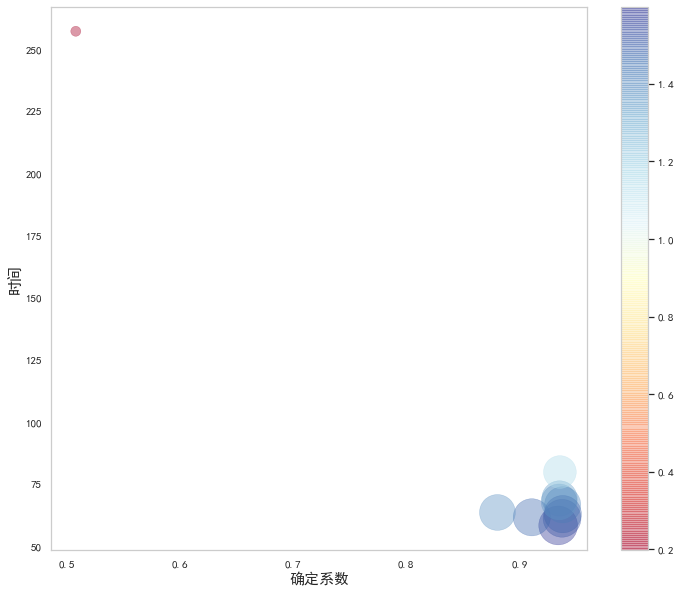
\includegraphics[width=0.7\linewidth]{pic/screenshot014}
%	\caption{}
%	\label{fig:screenshot014}
%\end{figure}

\begin{table}[H]
	\centering
	\caption{10种调参模型的模型效果评判}
	\label{tab:my-table1}
	\begin{tabular}{rrrrr}
		\hline
		序号& & \multicolumn{1}{c}{r} & \multicolumn{1}{c}{T / ms} & \multicolumn{1}{c}{s} \\ \hline
		1 & & 0.9342                & 58.4025               & 1.5996                \\
		2&  & 0.9354                & 69.2492               & 1.3507                \\
		3 & & 0.9376                & 61.2784               & 1.5301                \\
		4  && 0.9109                & 61.6864               & 1.4767                \\
		5  && 0.9382                & 66.7216               & 1.4061                \\
		6  && 0.9383                & 62.9502               & 1.4905                \\
		7  && 0.5082                & 257.0746              & 0.1977                \\
		8  && 0.8806                & 63.6268               & 1.3839                \\
		9  && 0.9350                & 67.8759               & 1.3776                \\
		10 && 0.9357                & 79.8768               & 1.1715                \\ \hline
	\end{tabular}
\end{table}


\subsection{每个GRU单元中偏置b初始化为1\cite{jozefowicz2015empirical}}

由上一小节,我们得出:模型1,即GRU(20)$ \rightarrow $Dropout(0.2)$ \rightarrow $GRU(20)

\noindent$ \rightarrow $Dropout(0.2)$ \rightarrow $Dense的效果最好,因此此后都在此基础上修改。

此处将所有偏置b初始化为1,模型代码更改为:
\begin{lstlisting} [language=Matlab]
function layers=get_gru_net(wd)
	numFeatures=wd;
	numResponses=1;
	numHiddenUnits=20;
	
	layers=[sequenceInputLayer(numFeatures)
	gruLayer(numHiddenUnits,"BiasInitializer","ones")
	dropoutLayer(0.2)
	gruLayer(numHiddenUnits,"BiasInitializer","ones")
	dropoutLayer(0.2)
	fullyConnectedLayer(numResponses)
	regressionLayer];
end
\end{lstlisting}

评判模型效果,结果如下:$  T=60.573ms, \ r=0.93623,\ s=\dfrac{100r}{T}=1.54562$。综合效果不如原本模型,但其训练收敛速度较原本模型有较大提升(loss收敛至$ 3\times 10^{-4} $只需要40轮)。
\subsection{全链接层使用Highway Network代替\cite{srivastava2015highway}}

Highway Network的灵感来自“解决RNN的问题,提出的LSTM结构”也就是加入“门”结构。

对于一般网络,其输出可以用如下公式表示:
\begin{equation}\label{normal}
	y=H(x,W^H)
\end{equation}

而在Highway Network中,我们定义一个新网络T,此时输出化为:

\begin{equation}\label{HeightWay}
	y=H(x,W^H)\cdot T(x,W^T)+x\cdot (1-T(x,W^T))
\end{equation}


此时不难发现,对于特殊的T值,该输出有如式\ref{HW_Proformance}的表现:

\begin{equation}\label{HW_Proformance}
	y=
	\left\{\begin{matrix} 
	x& &T=0\\  
	H&(x,W^H)\qquad\qquad&T=1
\end{matrix}\right. 
\end{equation}

若假设所有的门T的均值为0.5的话,就是把所有的原始信息一半激活,一半不变直接输入下一层,这样一来则保留了很多信息。同时反向传播的时候,可以让更多的(梯度)信息直接回流到输入,而不需要经过一个非线性转化。

由于笔者没有找到Matlab中如何自定义网络,因此此部分在Python中使用tensorflow实现。

使用tensorflow定义Highway单元,其代码如下:

\begin{lstlisting} [language=Python]
def highway(x, size, activation, carry_bias=-1.0):
	W_T = tf.Variable(tf.truncated_normal([size, size], stddev=0.1), name="weight_transform")
	b_T = tf.Variable(tf.constant(carry_bias, shape=[size]), name="bias_transform")

	W = tf.Variable(tf.truncated_normal([size, size], stddev=0.1), name="weight")
	b = tf.Variable(tf.constant(0.1, shape=[size]), name="bias")

	T = tf.sigmoid(tf.matmul(x, W_T) + b_T, name="transform_gate")
	H = activation(tf.matmul(x, W) + b, name="activation")
	C = tf.sub(1.0, T, name="carry_gate")

	y = tf.add(tf.mul(H, T), tf.mul(x, C), "y")
	return y
\end{lstlisting}

更改后的神经网络架构为:GRU(20)$ \rightarrow $Dropout(0.2)$ \rightarrow $GRU(20)$ \rightarrow $ 

\noindent Dropout(0.2)$ \rightarrow $Highway   。此时对此模型进行评估可以得到如下结果:
$  T=50.387ms, \ r=0.93382,\ s=\dfrac{100r}{T}=1.8536
 $
 
相较于原本模型:$  T=58.402ms, \ r=0.93418,\ s=\dfrac{100r}{T}=1.5996
$有较大幅度的提升。


\section{结果}


由于Matlab中无法定义highway网络,因此Matlab使用结果3.4.3中模型得出结果。结果如图\ref{fig:screenshot021}所示。
\begin{figure}[H]
	\centering
	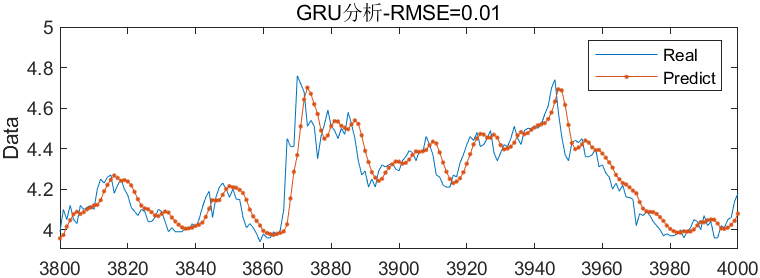
\includegraphics[width=1\linewidth]{pic/screenshot021}
	\caption{MATLAB中使用3.4.3中模型得出结果}
	\label{fig:screenshot021}
\end{figure}


\begin{figure}[H]
	\centering
	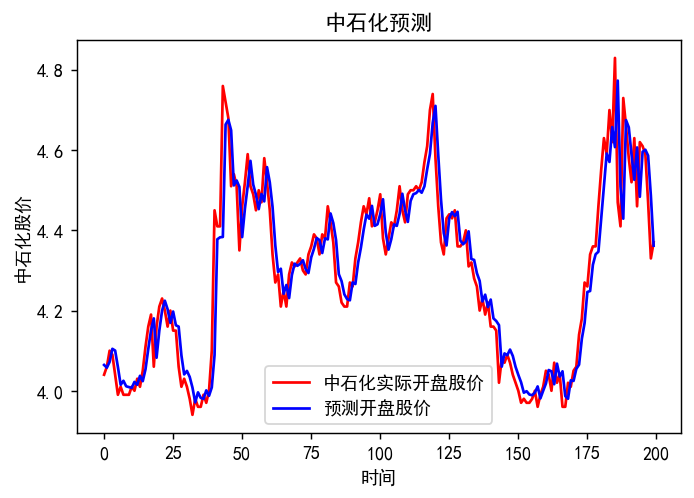
\includegraphics[width=0.7\linewidth]{pic/screenshot022}
	\caption{Python中使用3.4.4模型得出的结果}
	\label{fig:screenshot022}
\end{figure}

在Python中,把全链接层换为Highway层,得出结果如图\ref{fig:screenshot022}所示。
\chapter{股市K线预测}

\section{K线图的画法}

 K线图源于日本,被当时日本米市的商人用来记录米市的行情与价格波动,后因其细腻独到的标画方式而被引入到股市及期货市场。下面来实现茅台预测日K线的描绘。
 \begin{figure}[H]
 	\centering
 	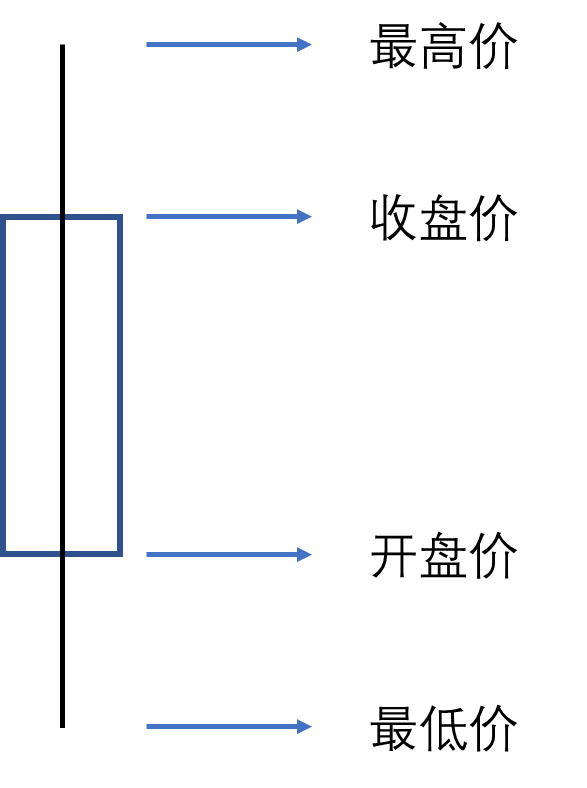
\includegraphics[width=0.3\linewidth]{pic/screenshot030}
 	\caption{K线图画法}
 	\label{fig:screenshot030}
 \end{figure}
 

日K线有如下特点\cite{Klinesgv}:
\begin{enumerate}
	\item 日K线为股票当日的开盘价、最高价、最低价、收盘价情况
	\item 阳线为红色柱体,表示股票上涨情况
	\item 阴线为绿色柱体,表示股票下跌情况
\end{enumerate}

\section{K线数据的准备}

K线数据需要:
\begin{enumerate}
	\item 开盘价
	\item 最高价
	\item 最低价
	\item 收盘价
\end{enumerate}

使用上一节中的模型对此4组数据进行预测并保存到Xlsx中,方便在绘制的时候调用。

\section{Matlab中K线的实现\cite{Kline}}

Matlab中有 candle.m函数可以实现蜡烛图的绘制,但其结果如下:
\begin{figure}[H]
	\centering
	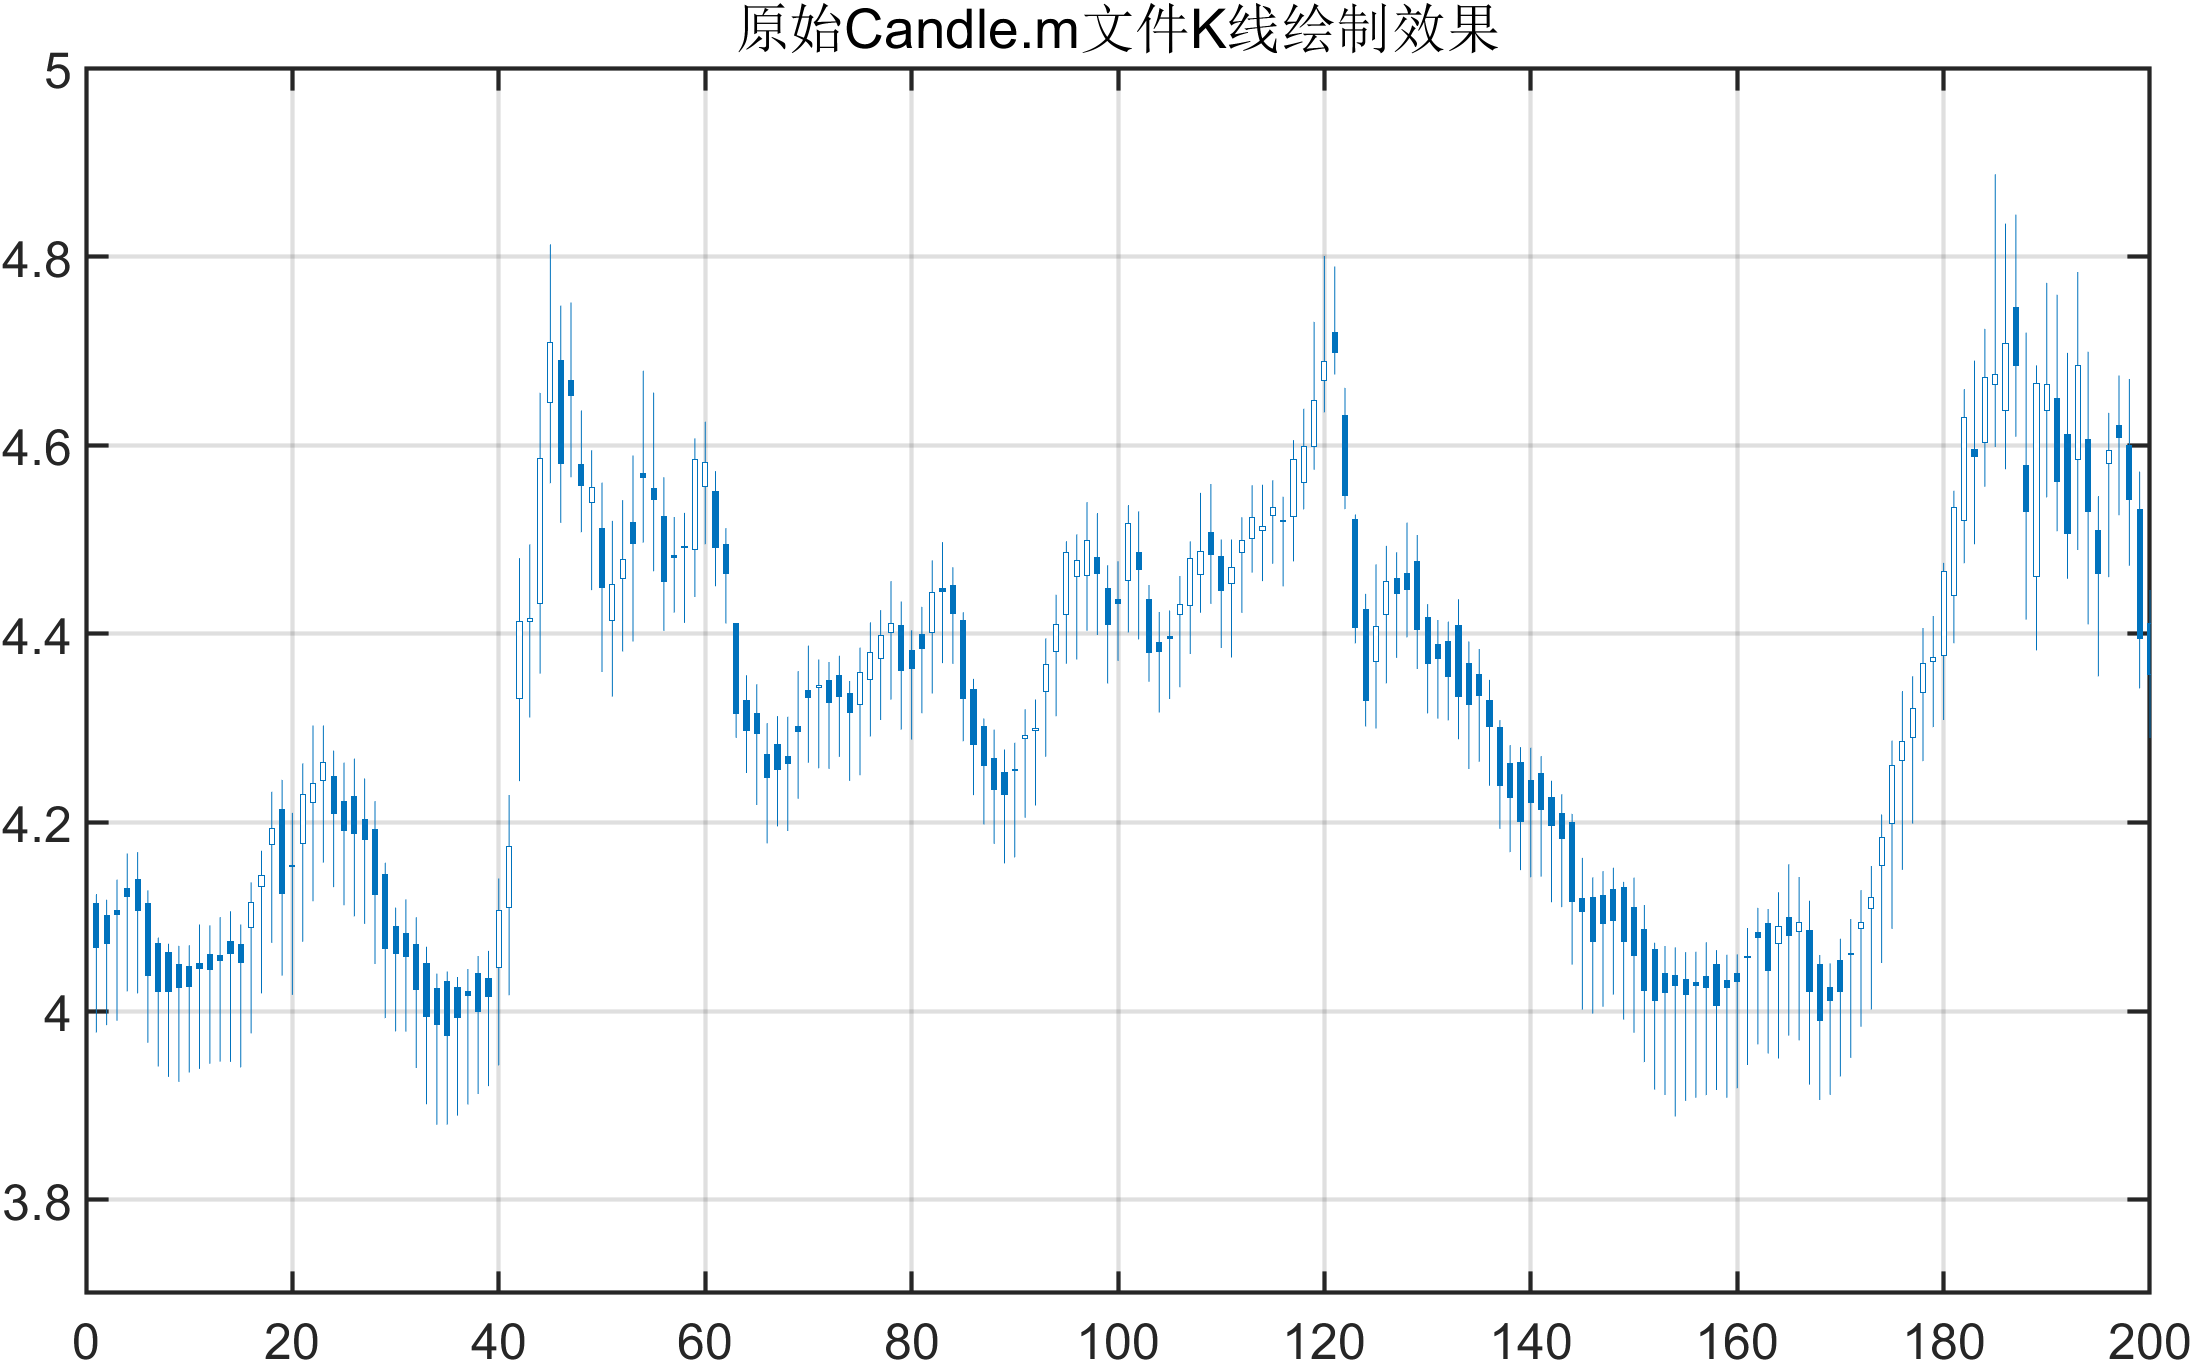
\includegraphics[width=0.8\linewidth]{pic/screenshot031}
	\caption{原始 Candle.m文件K线绘制效果}
	\label{fig:screenshot031}
\end{figure}

虽然已经有了大体的框架,但与我们常用的K线图还是有些许不同,因此需要对脚本进行修改,加入颜色,使其更加直观。
\begin{enumerate}
	\item 根据开盘价和收盘价设置响应的颜色,其代码如下:
	\begin{lstlisting} [language=Matlab]
kk=indexVertical(:,find(op > cl));
kkk=hiloVertical(:,find(op > cl));
hh1=plot(ax,kk(:),kkk(:),'color',[0 150/255 0],'LineWidth',1,'AlignVertexCenters','on');
hold on;
kk=indexVertical(:,find(op <= cl));
kkk=hiloVertical(:,find(op <= cl));
hh2=plot(ax,kk(:),kkk(:),'r-','LineWidth',1,'AlignVertexCenters','on');
h = [hh1 hh2];
	\end{lstlisting}
	
		\item 判断需要填的颜色,其代码如下:
	\begin{lstlisting} [language=Matlab]
filledIndex = ones(numObs, 1);
filledIndex(op <= cl) = 2;
	\end{lstlisting}
	\item 修改涨跌颜色(涨使用红色,跌使用绿色),其代码如下:
	\begin{lstlisting} [language=Matlab]
colorSet = {[0 150/255 0],'red'};
	\end{lstlisting}
	\item 修改边框颜色,
	其代码修改如下:
\begin{lstlisting} [language=Matlab]
for i = 1 : numObs
	h(i+2) = fill(ax, ...
		[indexLeft(i); indexLeft(i); indexRight(i); indexRight(i)], ...
		[op(i); cl(i); cl(i); op(i)],colorSet{filledIndex(i)},'Edgecolor',colorSet{filledIndex(i)}, ...
		'AlignVertexCenters', 'on');
end	
\end{lstlisting}
	
\end{enumerate}

如此修改后即可实现K线的绘制。


\section{结果}
\begin{figure}[H]
	\centering
	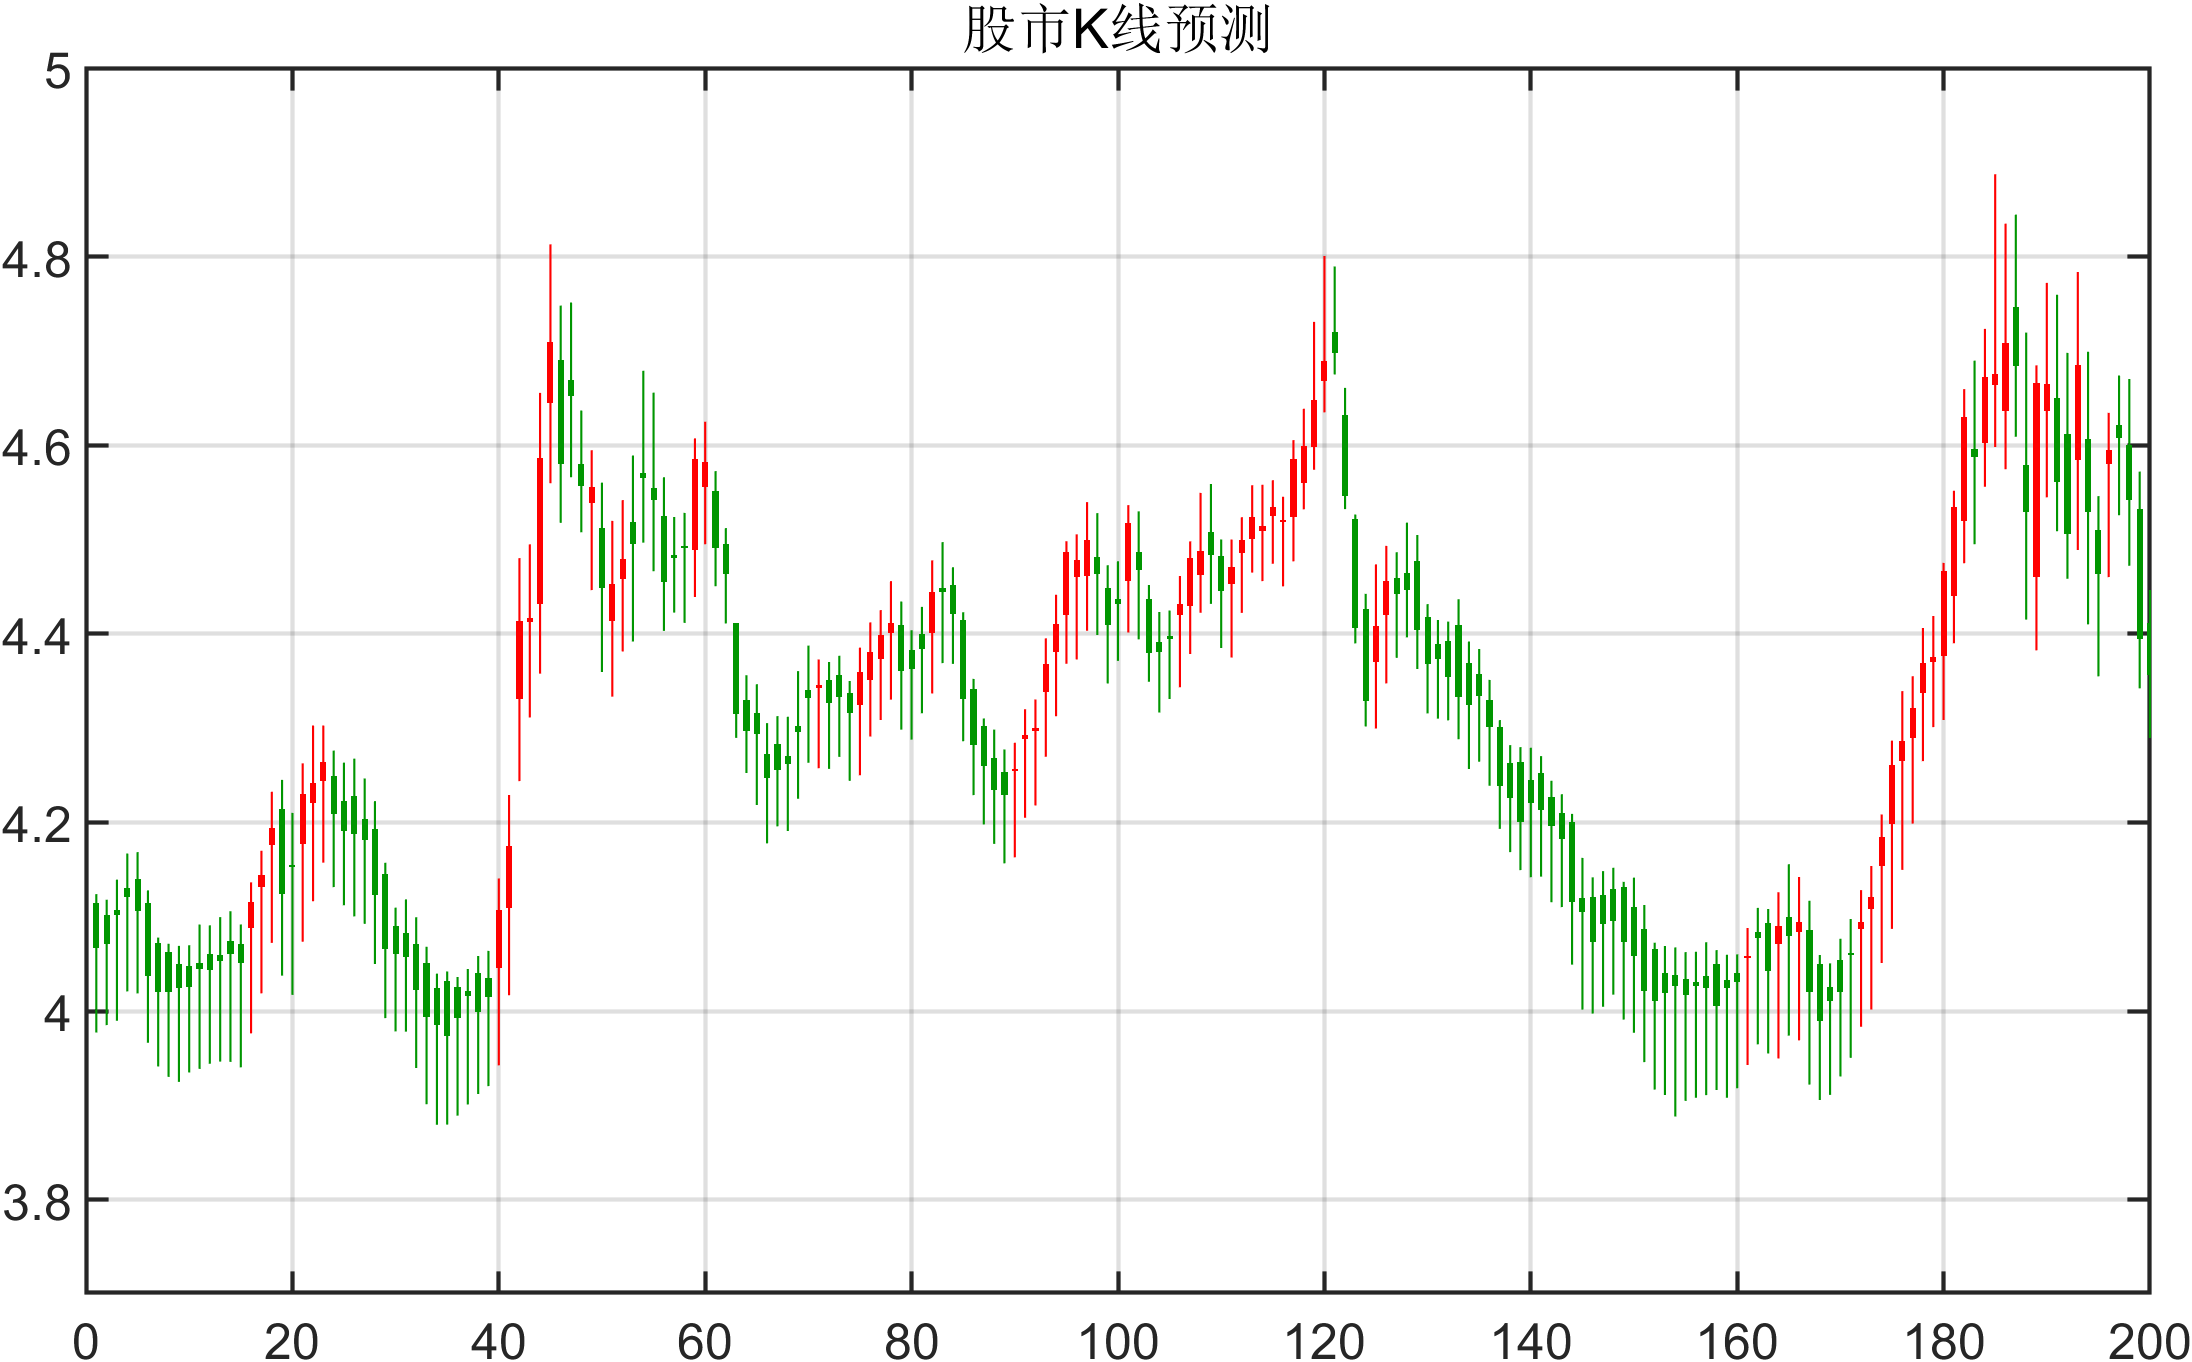
\includegraphics[width=0.8\linewidth]{pic/screenshot029}
	\caption{股市K线预测}
	\label{fig:screenshot029}
\end{figure}








\chapter{实验总结}
在这次课程设计中,我们运用课堂上所学习到的知识和课外搜集到的资料,用MATLAB实现了对股市的预测。在设计过程中,我们遇到了以下几个问题:
\begin{enumerate}
	\item 不会使用MATLAB的深度学习工具箱。
\item 代码实现上,一开始忘记反归一化,结果中出现负数。
\item 刚开始训练100次,用了78分钟,效率低。
\end{enumerate}

通过资料查询、代码检查和讨论分析,我们把上述问题都解决了。以下是我们的解决方法:
\begin{enumerate}
	\item 通过查阅官方文档和网上其他人的使用例子,我们学会了使用MATLAB的深度学习工具箱。
\item 通过检查代码,我们发现是忘记反归一化导致负数的出现。反归一化后,不出现负数。
\item 尝试更换电脑进行训练,训练时间缩短,效率提高。
\end{enumerate}

通过这次课程设计,我们学习到了更多有关MATLAB的知识,如RNN网络、LSTM结构、GRU网络的结构和特点;深度学习工具箱的使用;GRU神经网络在MATLAB中的搭建等。同时,这次课程设计也让我们对MATLAB的使用更加熟练,提高了我们的动手能力和团队协作能力。

%\appendix
%\chapter*{结论}\addcontentsline{toc}{chapter}{\hspace{-1em}结论}
%
%
%
%
%\chapter*{参考文献}\addcontentsline{toc}{chapter}{\hspace{-1em}参考文献}
%\bibliographystyle{unsrt}
\bibliographystyle{gbt7714-numerical}
\bibliography{ref}



\end{document}
